% !Mode:: "TeX:UTF-8"
% !TEX program  = xelatex

%\documentclass{cumcmthesis}
\documentclass[withoutpreface,bwprint]{cumcmthesis} %去掉封面与编号页

\usepackage{url}   % 网页链接
\usepackage{subcaption} % 子标题
\title{全国大学生数学建模竞赛编写的 \LaTeX{} 模板}
\tihao{A}
\baominghao{4321}
\schoolname{XX大学}
\membera{}
\memberb{向左}
\memberc{哈哈}
\supervisor{老师}
\yearinput{2017}
\monthinput{08}
\dayinput{22}

\title{一维非齐次热传导方程的Crank-Nicolson格式}
\begin{document}
	\maketitle
	~\\
	~\\
	
	作业:
	
	$$
	\left\{
	\begin{array}{lcl}
	\dfrac{\partial{u}}{\partial{t}}=\dfrac{\partial^{2}{u}}{\partial{x}^{2}} &,&0 \leq x \leq 1,0 \leq t \leq 1 \\
	
	u(x,0)=e^x &, & 0 \leq x \leq 1 \\
	
	u(0,t)=e^t,u(1,t)=e^{1+t},&, &0 \leq t \leq 1
	\end{array}
	\right.
	$$

该问题的精确解为$ u(x,t)=e^{x+t}$.

定义误差为$$ E_{\infty}(h,\tau)=\max \limits_{1 \leq i \leq m-1 \atop 1 \leq k \leq n } |u(x_{i},t_{k})-u_{k}^k)| $$

用Crank-Nicolson格式求下述问题的数值解并对数值解、精度和误差阶进行相应的数值分析。


~\\
~\\

解:

将xm等分,将tn等分, 记$h=\dfrac{1}{m},\tau=\dfrac{1}{n}$

$x_i=ih,0 \leq i \leq m$

$t_k=k \tau,0 \leq k \leq n$

Crank-Nicolson差分格式为
\begin{equation*}
\left\{
\begin{array}{lcl}
\dfrac{u_i^{k+1}-u_i^{k}}{\tau}=\dfrac{1}{2}(\dfrac{u_{i+1}^k-2u_{i}^{k}+u_{i-1}^k}{h^2}+\dfrac{u_{i+1}^{k+1}-2u_{i}^{k+1}+u_{i-1}^{k+1}}{h^2})+f(x_i,t_{k+\frac{1}{2}}) \\
u_i^0=e^{x_{i}} \\
u_0^k=e^{t_k},u_m^k=e^{1+t_k} \\
\end{array}
\right.
\end{equation*}

其中,$1 \leq i \leq m-1,1 \leq k \leq n,\gamma=\dfrac{\tau}{h^2}$

$f(x_i,t_k)=0$



写成矩阵形式$A_1u^{k+1}=A_2u^k+f$

其中
$$
A_1=
\begin{bmatrix}
1+\gamma & -\dfrac{\gamma}{2} \\
-\dfrac{\gamma}{2} & 1+\gamma & -\dfrac{\gamma}{2} \\
& \ddots & \ddots & \ddots \\
& & 	-\dfrac{\gamma}{2} & 1+\gamma
\end{bmatrix}
$$

$$
A_2=
\begin{bmatrix}
1-\gamma & \dfrac{\gamma}{2} \\
\dfrac{\gamma}{2} & 1-\gamma & \dfrac{\gamma}{2} \\
& \ddots & \ddots & \ddots \\
& & 	\dfrac{\gamma}{2} & 1-\gamma
\end{bmatrix}
$$

$$u^k=[u_1^k,u_2^k,\cdots,u_{m-1}^k]^T$$.

$$f=[\dfrac{\gamma}{2}(u_0^k+u_0^{k+1}),0,0\cdots,0,\dfrac{\gamma}{2}(u_m^k+u_m^{k+1})]^T$$.


解方程,由第k层的值,能够求出第k+1层的值。

~\\
~\\


\textbf{解题程序运行于Matlab 2018a.}

当$\tau=\dfrac{1}{10},h=\dfrac{1}{10}$时,t=1处的数值解和精确解见图\ref{fig:f1},从图像上看很接近。
\begin{figure}
	\centering
	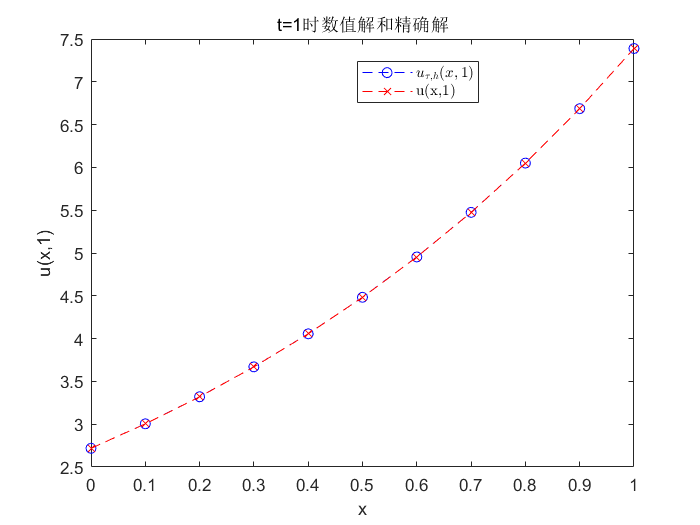
\includegraphics[width=0.7\linewidth]{figures/f1}
	\caption{t=1处的数值解和精确解}
	\label{fig:f1}
\end{figure}

当$\tau=\dfrac{1}{10},h=\dfrac{1}{10}$时,取x=0.5,不同t处的值见表\ref{tab:1},
当层数越深时,误差越大,这是因为,每一次由k层求解k+1层时都有误差,随着t的增大,误差不断累积,越来越大,
到t=1处误差变得最大。
% Table generated by Excel2LaTeX from sheet 'Sheet1'
% Table generated by Excel2LaTeX from sheet 'Sheet1'
\begin{table}[htbp]
	\centering
	\caption{x=0.5时,不同t处的数值解、精确解和误差}
	\begin{tabular}{ccccc}
		\toprule[1.5pt]
		k     & t     & 数值解   & 精确解   & 误差 \\
		\midrule[1pt]
		1     & 0.1   & 1.822349  & 1.822119  & 2.3053E-04 \\
		2     & 0.2   & 2.014105  & 2.013753  & 3.5224E-04 \\
		3     & 0.3   & 2.225953  & 2.225541  & 4.1241E-04 \\
		4     & 0.4   & 2.460072  & 2.459603  & 4.6922E-04 \\
		5     & 0.5   & 2.718802  & 2.718282  & 5.2042E-04 \\
		6     & 0.6   & 3.004743  & 3.004166  & 5.7700E-04 \\
		7     & 0.7   & 3.320755  & 3.320117  & 6.3794E-04 \\
		8     & 0.8   & 3.670002  & 3.669297  & 7.0507E-04 \\
		9     & 0.9   & 4.055979  & 4.055200  & 7.7949E-04 \\
		10    & 1     & 4.482550  & 4.481689  & 8.6123E-04 \\
		\bottomrule[1.5pt]
	\end{tabular}%
	\label{tab:1}%
\end{table}%


取不同$\tau$ 和 $h$时,t=1处的误差见图\ref{fig:f2},步长越小,误差也越小。
\begin{figure}
	\centering
	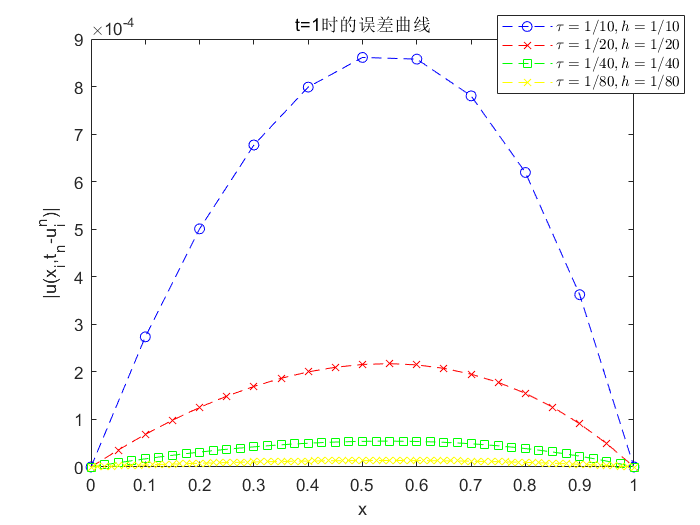
\includegraphics[width=0.7\linewidth]{figures/f2}
	\caption{不同步长下的误差}
	\label{fig:f2}
\end{figure}


分别用向后Euler格式和Crank-Nicolson格式,取不同步长时最大误差和最大误差的比值见表\ref{tab:2},
可知,用向后Euler格式, $\tau$变为原来的4倍,$h$变为原来的2倍,误差会变为原来的4倍,
符合$O(\tau+h^2)$的截断误差;	而Crank-Nicolson格式, $\tau$变为原来的2倍,$h$变为原来的2倍,误差会变为原来的4倍,
符合$O(\tau^2+h^2)$的截断误差,精度高于向后Euler格式。

% Table generated by Excel2LaTeX from sheet 'Sheet1'
% Table generated by Excel2LaTeX from sheet 'Sheet1'
\begin{table}[htbp]
	\centering
	\caption{不同步长的最大误差和最大误差的比}
	\begin{tabular}{ccc|ccc}
		\toprule[1.5pt]
		\multicolumn{3}{c}{Crank-Nicolson格式} & \multicolumn{3}{c}{向后Euler格式} \\
		\midrule[1pt]
		$h,\tau$   & $E_{\infty}(h,\tau)$ & $E_{\infty}(2h,2\tau)/E_{\infty}(h,\tau)$ & 	$h,\tau$   & $E_{\infty}(h,\tau)$ & $E_{\infty}(2h,4\tau)/E_{\infty}(h,\tau)$ \\
		1/10,1/10 & 8.61E-04 & *     & 1/100,1/10 & 3.01E-03 & * \\
		1/20,1/20 & 2.17E-04 & 3.962274  & 1/400,1/20 & 7.60E-04 & 3.956615 \\
		1/40,1/40 & 5.44E-05 & 3.998647  & 1/1600,1/40 & 1.90E-04 & 3.997046 \\
		1/80,1/80 & 1.36E-05 & 3.999657  & 1/6400,1/80 & 4.76E-05 & 3.999261 \\
		\bottomrule[1.5pt]
	\end{tabular}%
	\label{tab:2}%
\end{table}%


\end{document}